\chapter{Current state of Kdyby}

To be able to lay out the roadmap, first we have to know the current state of each Kdyby package, the original purpose and the current requirements. We will only review those packages that actually made it to production and at least one usable version was released.

I have created few GitHub repositories as a reminder for me to start working on some other web application development problems. I did start to work on some of them, for example on DoctrineForms, but it was never "officially released". We will not discuss these incomplete packages in this thesis.

\section{State of the project}

The most relevant problem is the compatibility with new versions of the libraries, that Kdyby integrates. There is \gls{nette} 2.4 and the 3.0 is being developed, but some of Kdyby packages support only \gls{nette} 2.2 or older.

The other problems appear only when you interact with the source code which is still really important for me as a maintainer and for the contributors. Also good maintainable code attracts more programmers to use it and contribute. But, there is no coding standard being enforced automatically on any package and no static analysis tool is checking the code. On the other hand almost all of the packages have unit and integration tests and linter checking the code for multiple versions of PHP.

\begin{figure}[h] \label{fig:php:supported-versions}
  \centering
    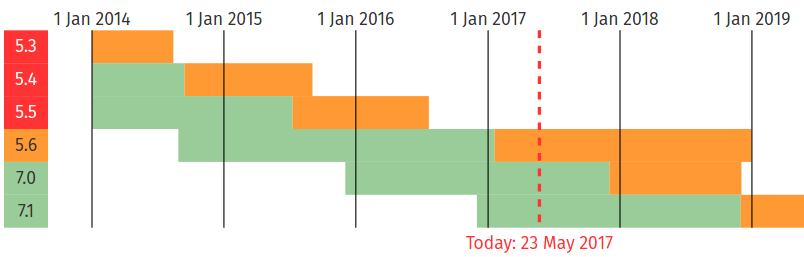
\includegraphics[width=1\textwidth]{src/assets/php-supported-versions.png}
  \caption{Supported PHP Versions. Green is active support, orange is security fixes only. Up-to-date version is at \url{http://php.net/supported-versions.php}}
\end{figure}

Most of the packages are compatible with PHP 5.4, but \fnurl{PHP 5.4 had end of life at \printdate{2015-09-03}}{http://php.net/eol.php} and is no longer supported by PHP developers.

The PHP 5.5 had end of life at \printdate{2016-06-21} and PHP 5.6 is currently in the phase of security fixes only and will have end of life at \printdate{2018-12-31}. As you can see on the graph~\ref{fig:php:supported-versions}, everyone should be migrating to PHP 7.0 by now, but it is not always as easy as simply upgrading PHP interpreter. The developer has to consider what PHP versions the libraries support, upgrade them first and then migrate the application.

\section{State of each package}

This section reviews each package separately, considers the original purpose and sums up the current state.

\hiddensubsection{Doctrine} \label{sec:state:doctrine}

\gls{kDoctrine} is an integration of \gls{doctrine} into Nette Framework.

\gls{doctrine} itself is separated into several packages, mainly \fnurl{doctrine/orm}{https://github.com/doctrine/doctrine2}, \fnurl{doctrine/common}{https://github.com/doctrine/common}, \fnurl{doctrine/annotations}{https://github.com/doctrine/annotations}, \fnurl{doctrine/cache}{https://github.com/doctrine/cache} and \fnurl{doctrine/collections}{https://github.com/doctrine/collections}. What started as a monolith integration in Kdyby, got separated into \gls{kEvents}~\ref{sec:state:events}, \gls{kConsole}~\ref{sec:state:console}, \gls{kAnnotations}~\ref{sec:state:annotations} and \gls{kDoctrineCache}~\ref{sec:state:doctrine-cache} for reusability.

Over the years, it cumulated a lot of responsibilities, that don't belong to it. I have already started extracting few of them in the past, for example an entity prototyping tool~\ref{sec:state:doctrine-magic-accessors}, collection utilities~\ref{sec:state:doctrine-collections-lazy}, \ref{sec:state:doctrine-collections-readonly} and helper for loading big SQL scripts to the database~\ref{sec:state:doctrine-dbal-batch-import}.

There is a big issue \fnurl{Chop up the package}{https://github.com/Kdyby/Doctrine/issues/238} that discusses what other parts should be separated and dropped completely.

New versions of Nette and \gls{doctrine} were released and completely new versions are being prepared, which the integration cannot be currently used with.

\hiddensubsection{Console} \label{sec:state:console}

\gls{kConsole} is an integration of Symfony Framework \lstinline{Console} Component, that allows for writing interactive CLI applications. \gls{kDoctrine}~\ref{sec:state:doctrine} depends on this package and is the reason this package exists.

There are tasks, that are better suited for console interaction, than a web interface. Among others, \gls{doctrine} has tools for generating a database schema from the entities metadata and there is a console command for it, that is written using Symfony \lstinline{Console}.

\hiddensubsection{Events} \label{sec:state:events}

\gls{kEvents} provides an event dispatcher~\ref{sec:theory:event-dispatcher} implementation for Nette Framework.

It started as an integration of \gls{doctrine} \lstinline{EventManager}, but then it evolved into a standalone system with support for lazy initialization of listeners and it also contains a naive bridge for Symfony Framework \lstinline{EventDispatcher} Component.

Creating such interchangeable eventing system turned out to be a mistake, because it is a maintenance hell. The systems should have stayed separate.

\hiddensubsection{Annotations} \label{sec:state:annotations}

\gls{kAnnotations} is a simple integration of doctrine/annotations into Nette Framework. It exists solely for the purposes of \gls{kDoctrine}.

\hiddensubsection{DoctrineCache} \label{sec:state:doctrine-cache}

Lorem ipsum.

\hiddensubsection{DoctrineMagicAccessors} \label{sec:state:doctrine-magic-accessors}

Lorem ipsum.

\hiddensubsection{DoctrineCollectionsReadonly} \label{sec:state:doctrine-collections-readonly}

Lorem ipsum.

\hiddensubsection{DoctrineCollectionsLazy} \label{sec:state:doctrine-collections-lazy}

Lorem ipsum.

\hiddensubsection{DoctrineDbalBatchImport} \label{sec:state:doctrine-dbal-batch-import}

Lorem ipsum.

\hiddensubsection{DoctrineForms} \label{sec:state:doctrine-forms}

Lorem ipsum.

\hiddensubsection{Curl} \label{sec:state:curl}

Lorem ipsum.

\hiddensubsection{CurlCaBundle} \label{sec:state:curl-ca-bundle}

Lorem ipsum.

\hiddensubsection{Autowired} \label{sec:state:autowired}

Lorem ipsum.

\hiddensubsection{FormsReplicator} \label{sec:state:forms-replicator}

Lorem ipsum.

\hiddensubsection{Translation} \label{sec:state:translation}

Lorem ipsum.

\hiddensubsection{Validator} \label{sec:state:validator}

Lorem ipsum.

\hiddensubsection{RabbitMq} \label{sec:state:rabbit-mq}

Lorem ipsum.

\hiddensubsection{Money} \label{sec:state:money}

Lorem ipsum.

\hiddensubsection{DoctrineMoney} \label{sec:state:doctrine-money}

Lorem ipsum.

\hiddensubsection{Aop} \label{sec:state:aop}

Lorem ipsum.

\hiddensubsection{Clock} \label{sec:state:clock}

Lorem ipsum.

\hiddensubsection{Redis} \label{sec:state:redis}

Lorem ipsum.

\hiddensubsection{ParseUseStatements} \label{sec:state:parse-use-statements}

Lorem ipsum.

\hiddensubsection{RedisActiveLock} \label{sec:state:redis-active-lock}

Lorem ipsum.

\hiddensubsection{TesterParallelStress} \label{sec:state:tester-parallel-stress}

Lorem ipsum.

\hiddensubsection{Monolog} \label{sec:state:monolog}

Lorem ipsum.

\hiddensubsection{ElasticSearch} \label{sec:state:elastic-search}

Lorem ipsum.

\hiddensubsection{DoctrineSearch} \label{sec:state:doctrine-search}

Lorem ipsum.

\hiddensubsection{Geocoder} \label{sec:state:geocoder}

Lorem ipsum.

\hiddensubsection{CsobPaygateNette} \label{sec:state:csob-paygate-nette}

Lorem ipsum.

\hiddensubsection{CsobPaymentGateway} \label{sec:state:csob-payment-gateway}

Lorem ipsum.

\hiddensubsection{Wkhtmltopdf} \label{sec:state:wkhtmltopdf}

Lorem ipsum.

\hiddensubsection{FakeSession} \label{sec:state:fake-session}

Lorem ipsum.

\hiddensubsection{RequestStack} \label{sec:state:request-stack}

Lorem ipsum.

\hiddensubsection{StrictObjects} \label{sec:state:strict-objects}

Lorem ipsum.

\hiddensubsection{Facebook} \label{sec:state:facebook}

Lorem ipsum.

\hiddensubsection{Google} \label{sec:state:google}

Lorem ipsum.

\hiddensubsection{Github} \label{sec:state:github}

Lorem ipsum.

\hiddensubsection{NettePhpServer} \label{sec:state:nette-php-server}

Lorem ipsum.

\hiddensubsection{TesterExtras} \label{sec:state:tester-extras}

Lorem ipsum.

\hiddensubsection{HtmlValidatorPanel} \label{sec:state:html-validator-panel}

Lorem ipsum.

\hiddensubsection{BootstrapFormRenderer} \label{sec:state:bootstrap-form-renderer}

Lorem ipsum.

\hiddensubsection{PayPalExpress} \label{sec:state:paypal-express}

Lorem ipsum.

\hiddensubsection{PresentersLocator} \label{sec:state:presenters-locator}

Lorem ipsum.

\hiddensubsection{SvgRenderer} \label{sec:state:svg-renderer}

Lorem ipsum.

\hiddensubsection{QrEncode} \label{sec:state:qr-encode}

Lorem ipsum.